\documentclass[a4paper, 12pt]{article}%тип документа

%отступы
\usepackage[left=2cm,right=2cm,top=2cm,bottom=3cm,bindingoffset=0cm]{geometry}

%Русский язык
\usepackage[T2A]{fontenc} %кодировка
\usepackage[utf8]{inputenc} %кодировка исходного кода
\usepackage[english,russian]{babel} %локализация и переносы

%Вставка картинок
\usepackage{wrapfig}
\usepackage{graphicx}
\graphicspath{{pictures/}}
\DeclareGraphicsExtensions{.pdf,.png,.jpg}

%оглавление
\usepackage{titlesec}
\titlespacing{\chapter}{0pt}{-30pt}{12pt}
\titlespacing{\section}{\parindent}{5mm}{5mm}
\titlespacing{\subsection}{\parindent}{5mm}{5mm}
\usepackage{setspace}

%Графики
\usepackage{multirow}
\usepackage{pgfplots}
\pgfplotsset{compat=1.9}

%Математика
\usepackage{amsmath, amsfonts, amssymb, amsthm, mathtools}

%Стиль страницы
\usepackage{fancyhdr}
\pagestyle{fancy}

\begin{document}

\begin{titlepage}

\begin{center}
%\vspace*{1cm}
\large\textbf{Московский Физико-Технический Институт}\\
\large\textbf{(государственный университет)}
\vfill
\line(1,0){430}\\[1mm]
\huge\textbf{Работа 3.6.1}\\
\line(1,0){430}\\[1mm]
\vfill
\large Сибгатуллин Булат, ФРКТ\\
\end{center}

\end{titlepage}
\fancyhead[L] {Работа 3.6.1}
\noindent \textbf{Цель работы: изучить спектральный состав периодических сигналов.} \\
\indent text\\
\noindent \textbf{В работе используются: анализатор спектраб генератор прямоугольных импульсов и сигналов специальной формы, осциллограф.} \\
\indent text

\section*{Описание работы}

В работе изучается спектральный состав периодических электрических сигналов различной формы: последовательность прямоугольных импульсов, последовательности цугов и амплитудно-модулированных колебаний. Спектры этих сигналлов наблюдаются с помощью анализатора спектра и сравниваются с рассчитанными теоретически.

Периодическая функция может быть представлена в виде бесконечного ряда гармонических функций - ряда Фурье:

\[f(t) = \sum\limits_{n = -\inf}^{\inf} c_n e^{in\omega_0 t} \quad \text{или} \quad 
f = \sum\limits_{n = 0}^{\inf} a_n \cos (n \omega_0 t + \phi_n ).\]

Здесь $\omega_0 = 2\pi /T$, где $T$ - период функции $f(t)$. Коэффициенты ${c_n}$ могут быть найдены по формулы:

\[c_n = \frac{1}{T} \int\limits_0^T f(t) e^{-in \omega_0 t} dt.\]

Наборы коэффициентов разложения в комплексной ${c_n}$ и действительной ${a_n, \phi_n}$ формах связаны соотношением:

\[a_n = 2 | c_n |, \quad \phi_n = \text{arg}c_n.\]

В качестве простейшего спектрального анализатора можно использовать высокодобротный колебательный контур с подстраиваемой ёмкостью или индуктивностью. Такой контур усиливает те гармоники входного сигнала $f(t)$, частота которых близка к резонансной $\nu_0 = 1/(2\pi \sqrt{LC}$ и практически не реагируют на частоты, далёкие от $\nu_0$. С точки зрения преобразования гармоник колебательный контур является узкополосным фильтром с шириной полосу пропускания порядка $\bigtriangleup \sim \nu_0/Q,$ где $Q = \frac{1}{R}\sqrt{\frac{L}{C}} \gg 1$ - его добротность. Амплитуда колебаний в контуре пропорциональна амплитуде $|c(\nu_0)|$ гармоники в спектре функции $f(t)$, частота которой совпадает с $\nu_0$. Таким образом, меняя резонансную частоту контура, можнно <<просканировать>> весь спектр входного сигнала.

\section*{Эскпериментальная установка}

\begin{figure}[h!]
\centering
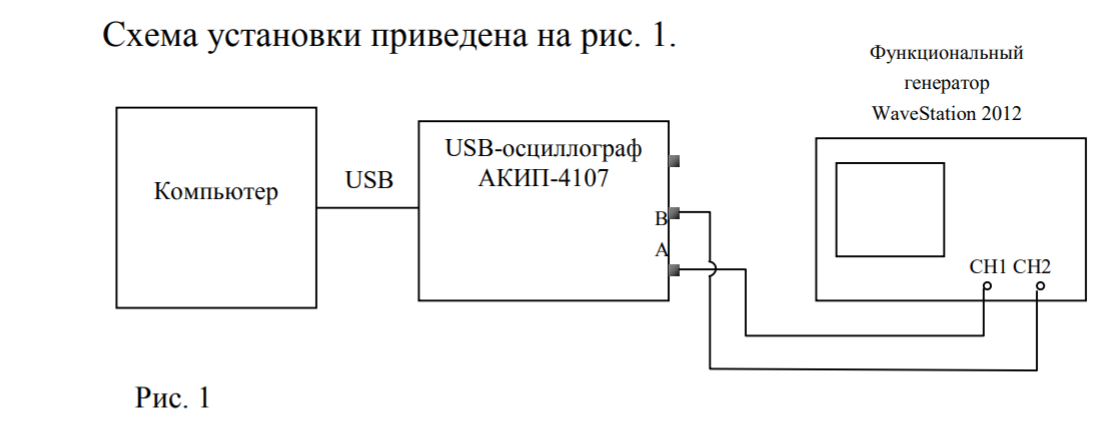
\includegraphics[scale=0.6]{images/scheme.png}
\label{fig:Image1}
\end{figure}

Функциональный генератор WaveStation 2012 позволяет сформировать два
различных электрических сигнала, которые выводятся на два независимых
канала – "CH1" и "CH2". Сигнал с канала "CH1" подается на вход "A", а
сигнал с канала "CH2" – на вход "B" USB-осциллографа. Затем эти сигналы подаются на вход компьютера через USB-соединение. При работе USBосциллографа в режиме осциллографа, на экране компьютера можно
наблюдать каждый из сигналов в отдельности, а также их произведение.
В режиме спектроанализатора можно наблюдать спектры этих сигналов. При включении функционального генератора, на его экране отображается информация о параметрах электрического сигнала.

\section*{Ход работы}

\subsection*{А}

\begin{enumerate}

\item Соберем и запустим усановку. Установим на анализаторе спектра режим работы с однократной разверткой и получим на экране спектр импульсов с параметрами:

а)$f_{\text{повт}} = 10^3$ Гц; $\tau = 25$ мкс; частотный масштаб $m_x = 5$ кГц/дел.

б)$f_{\text{повт}} = 10^3$ Гц; $\tau = 50$ мкс; частотный масштаб $m_x = 5$ кГц/дел.

в)$f_{\text{повт}} = 2\cdot 10^3$ Гц; $\tau = 25$ мкс; частотный масштаб $m_x = 5$ кГц/дел.

\begin{figure}[h!]
\centering
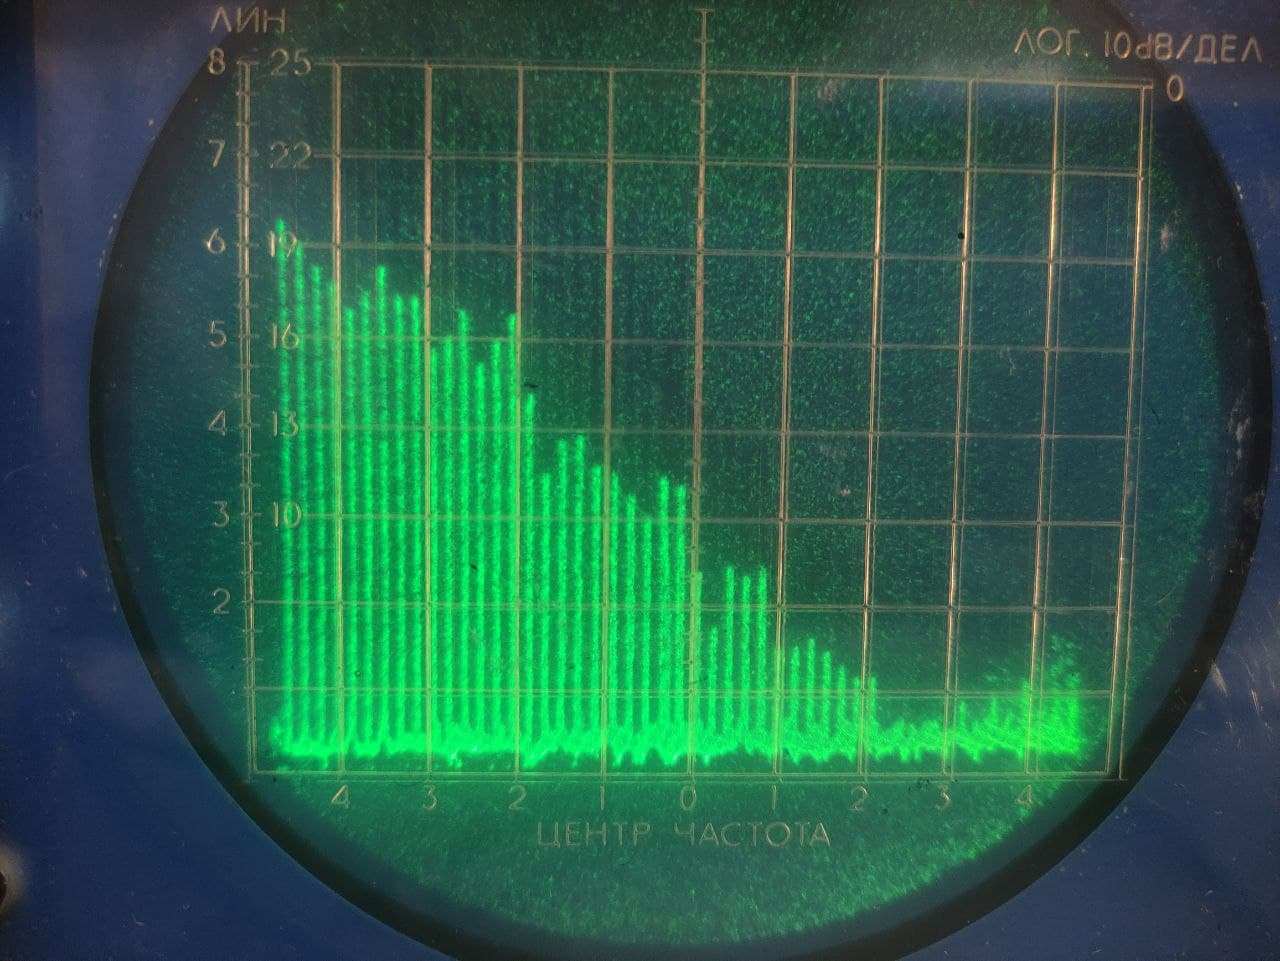
\includegraphics[scale=0.2]{images/25_1000-a.jpg}
\caption{$f_{\text{повт}} = 10^3$ Гц; $\tau = 25$ мкс}
\label{fig:Image1}
\end{figure}

\begin{figure}[h!]
\centering
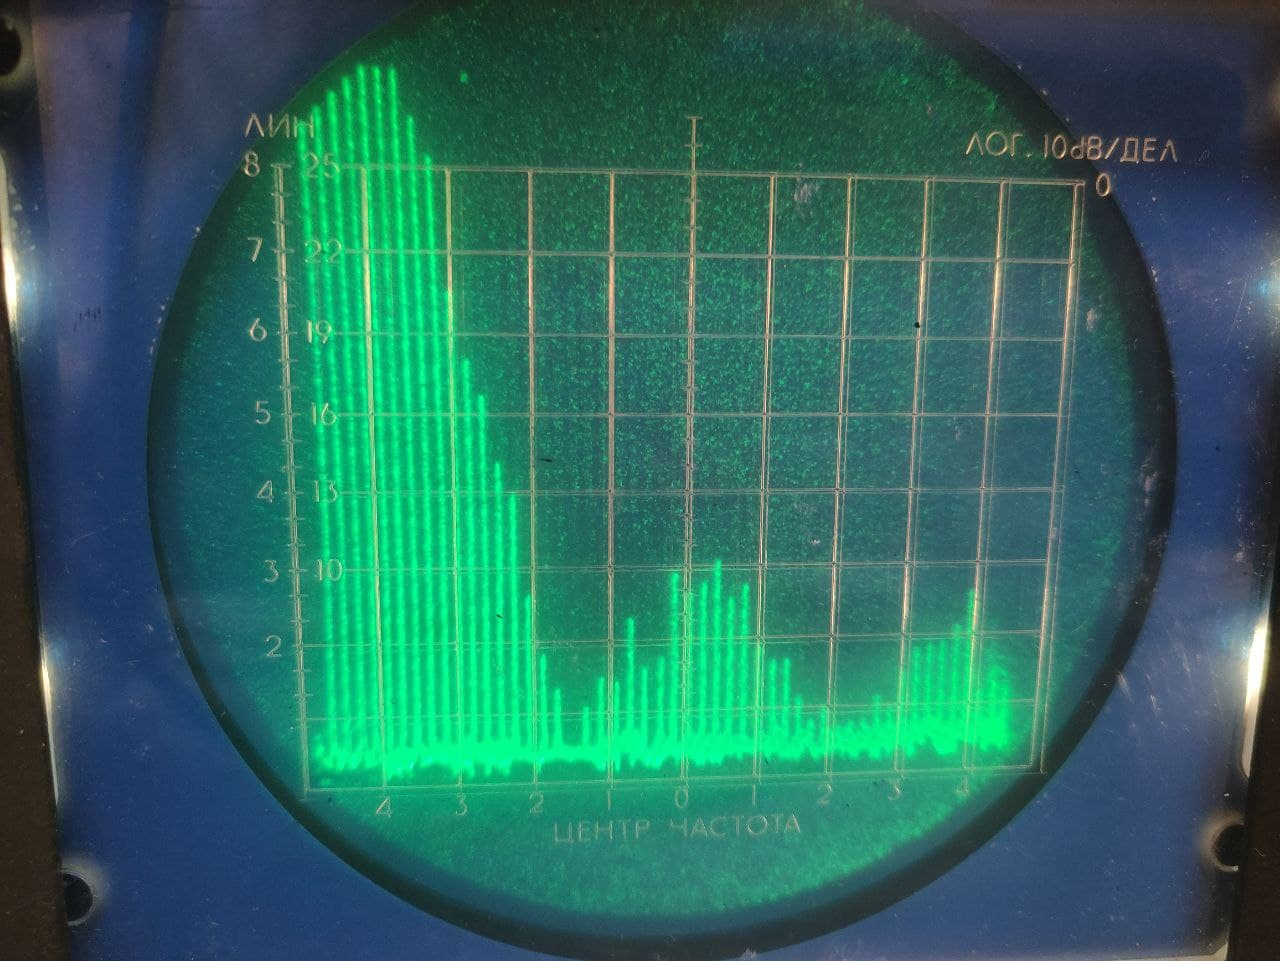
\includegraphics[scale=0.2]{images/50_1000-a.jpg}
\caption{$f_{\text{повт}} = 10^3$ Гц; $\tau = 50$ мкс}
\label{fig:Image1}
\end{figure}

\begin{figure}[h!]
\centering
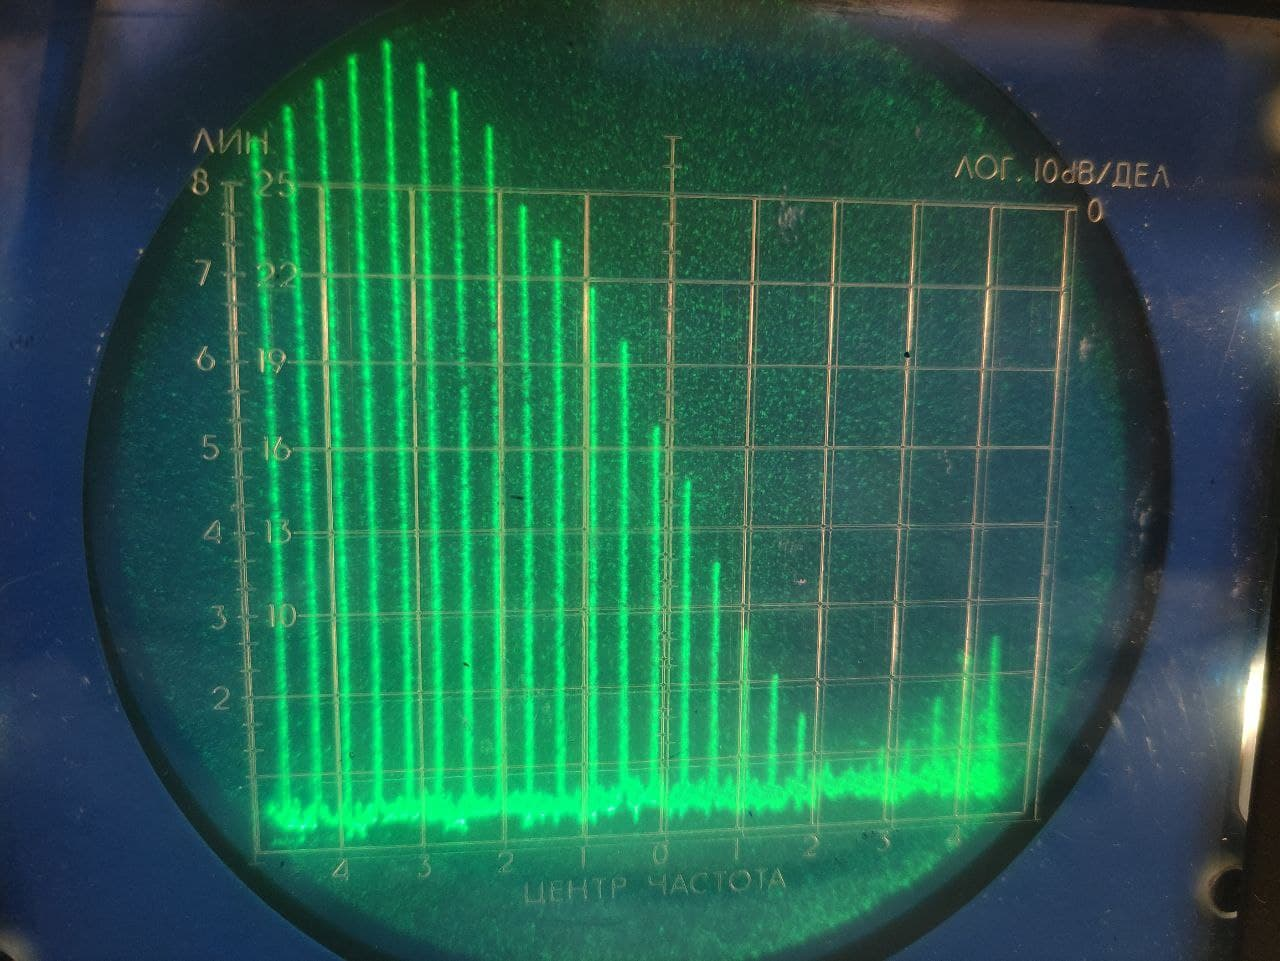
\includegraphics[scale=0.2]{images/25_2000-a.jpg}
\caption{$f_{\text{повт}} = 2\cdot 10^3$ Гц; $\tau = 25$ мкс}
\label{fig:Image1}
\end{figure}

\item Проведем измерения зависимости ширины спектра  от длительности импульса $\bigtriangleup \nu (\tau)$ при увеличении $\tau$ от 25 до 200 мкс. Запишем данные в таблицу.

\begin{figure}[h!]
\centering
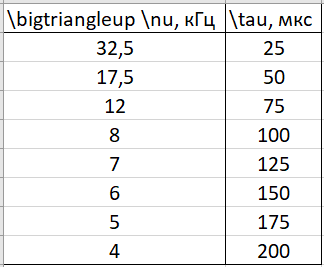
\includegraphics[scale=1.2]{images/table1.png}
\label{fig:Image1}
\end{figure}

\item Зарисуем спектры с параметрами $f_{\text{повт}} = 1$ кГц:

а) $\tau = 50$ мкс

б) $\tau = 100$ мкс

\begin{figure}[h!]
\centering
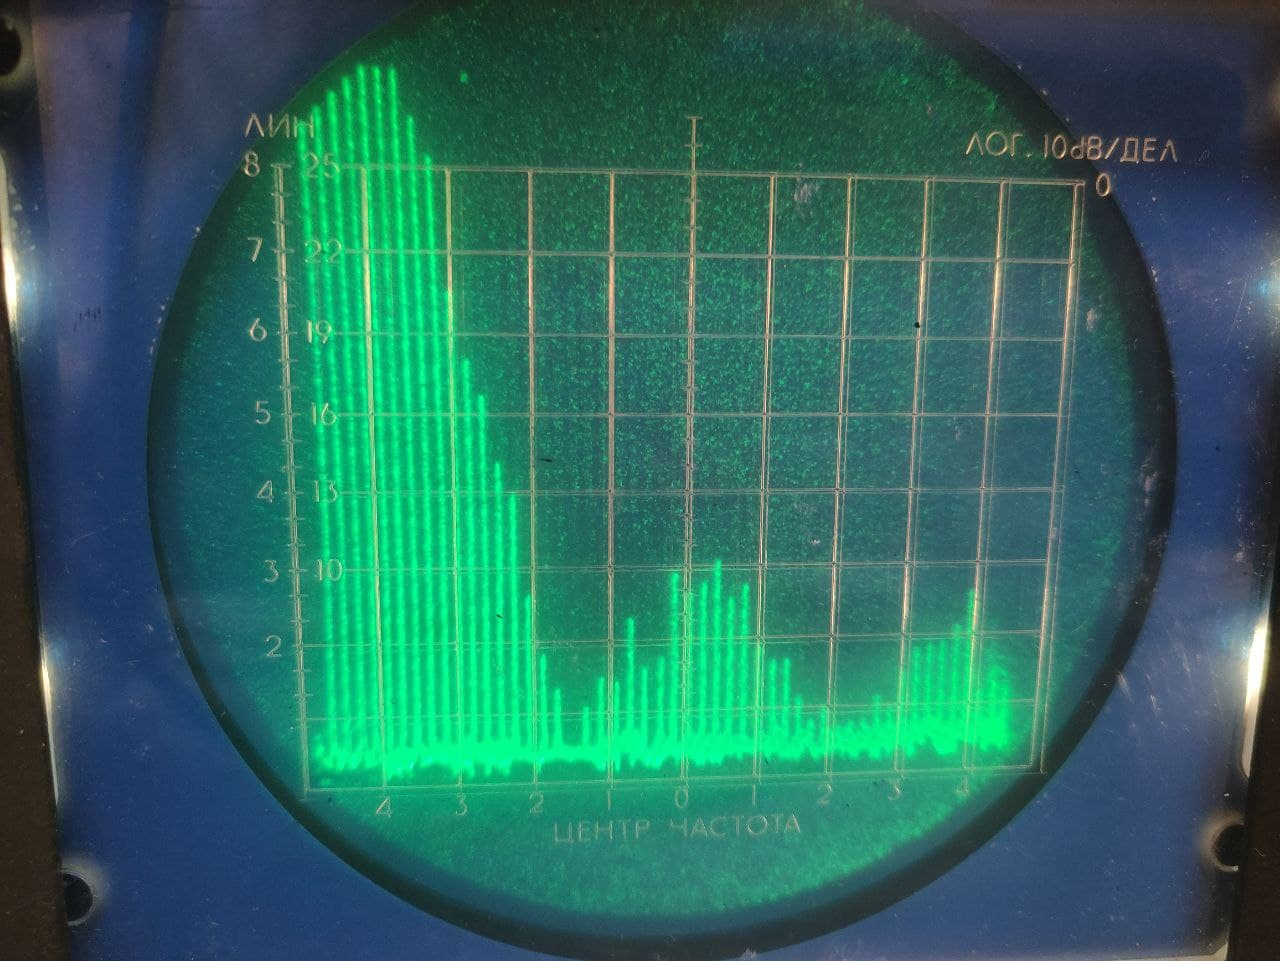
\includegraphics[scale=0.2]{images/50_1000-a.jpg}
\caption{$f_{\text{повт}} = 10^3$ Гц; $\tau = 50$ мкс}
\label{fig:Image1}
\end{figure}

\begin{figure}[h!]
\centering
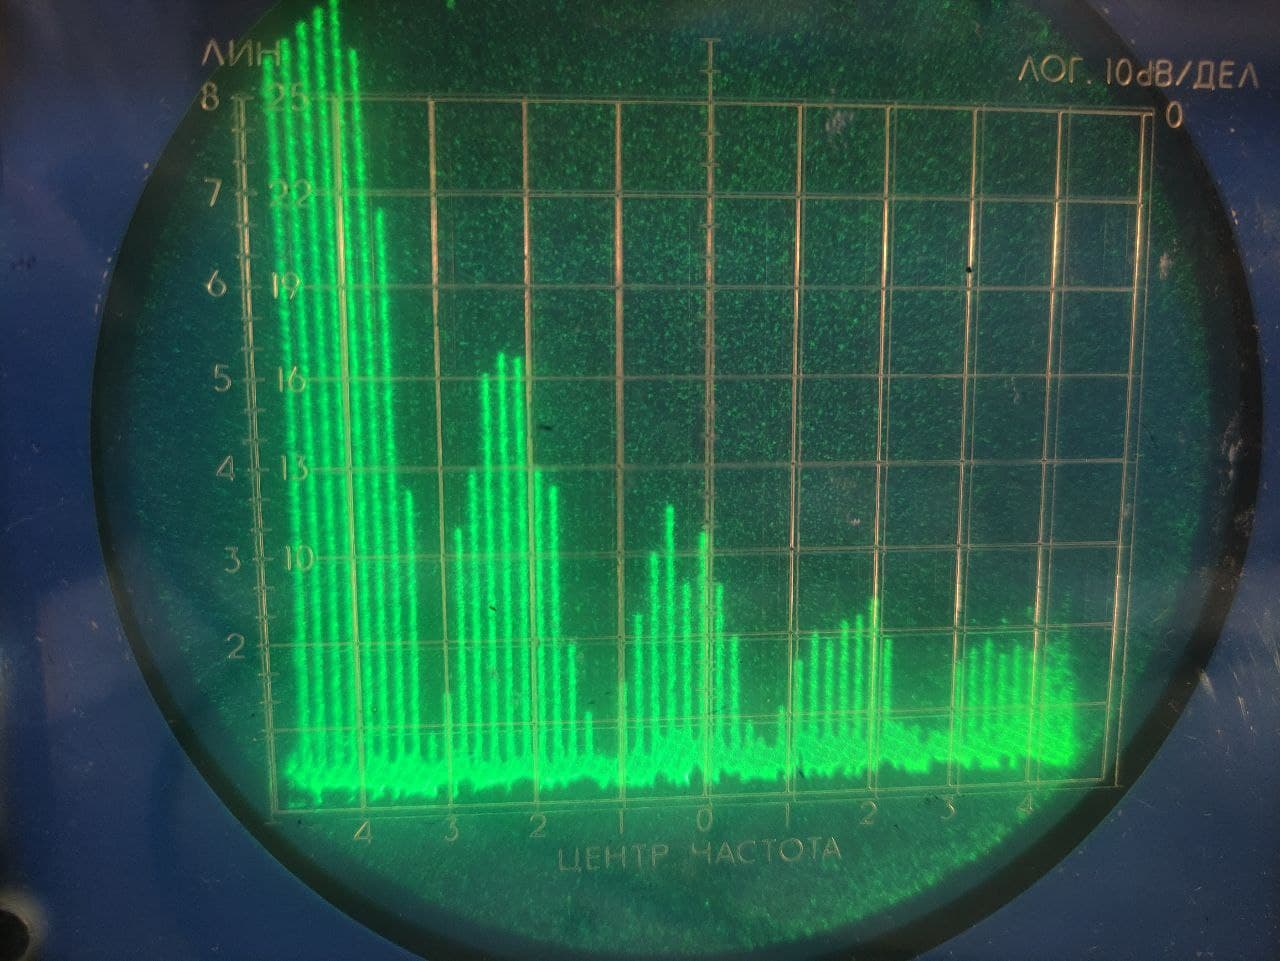
\includegraphics[scale=0.2]{images/100_1000-a.jpg}
\caption{$f_{\text{повт}} = 10^3$ Гц; $\tau = 100$ мкс}
\label{fig:Image1}
\end{figure}

\item Построим график зависимости $\bigtriangleup \nu (1/\tau)$ и по его наклону убедимся в том, что зависимость линейная:

\begin{figure}[h!]
\centering
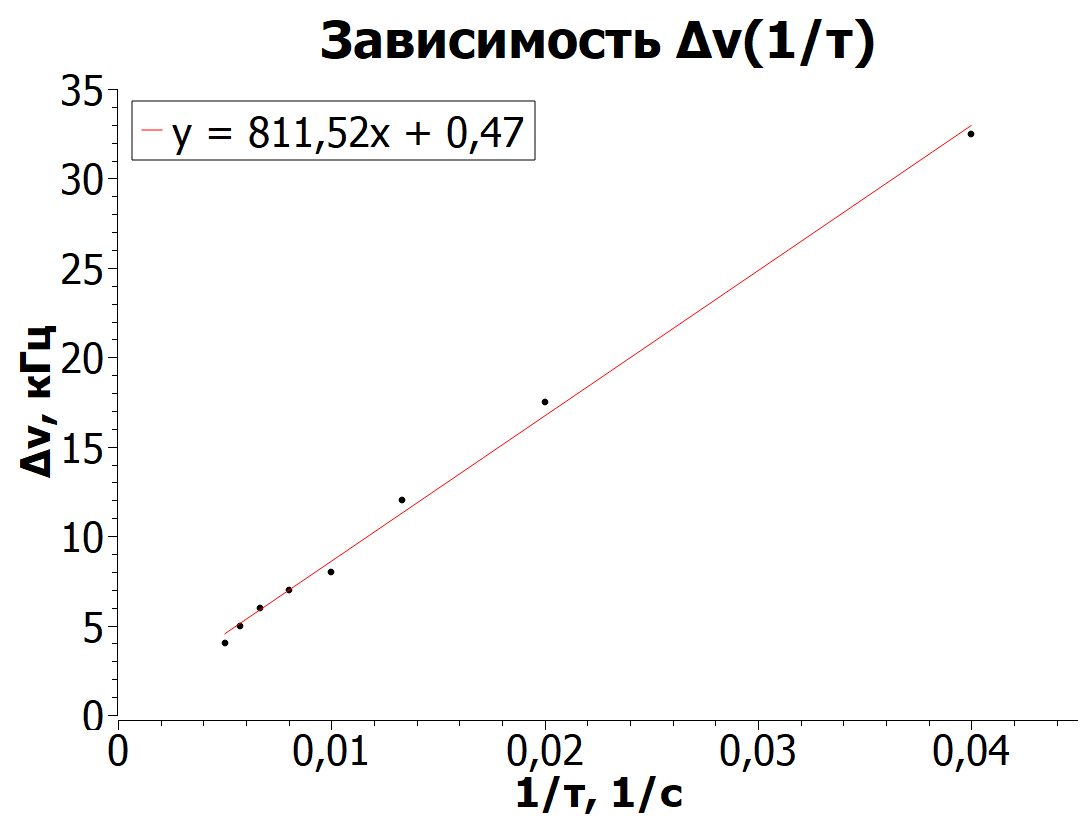
\includegraphics[scale=0.8]{images/graph1.png}
\label{fig:Image1}
\end{figure}

\end{enumerate}

\newpage

\subsection*{Б}

\begin{enumerate}

\item Изменим схему установки. Установим частоту несущей $\nu_0 = 25$ кГц и проанализируем как изменяется вид спектра:

а)при увеличении длительности импульса вдвое ($\tau = 50, 100$ мкс для $f_{\text{повт}} = 1$ кГц.

б)при изменении несущей частоты $\nu_0$ (на генераторе Г6-34 $\nu_0 = 25, 10$ или 40 кГц) при фиксированных значениях $f_{\text{повт}} = 1$ кГц, $\tau = 100$ мкс.

\begin{figure}[h!]
\centering
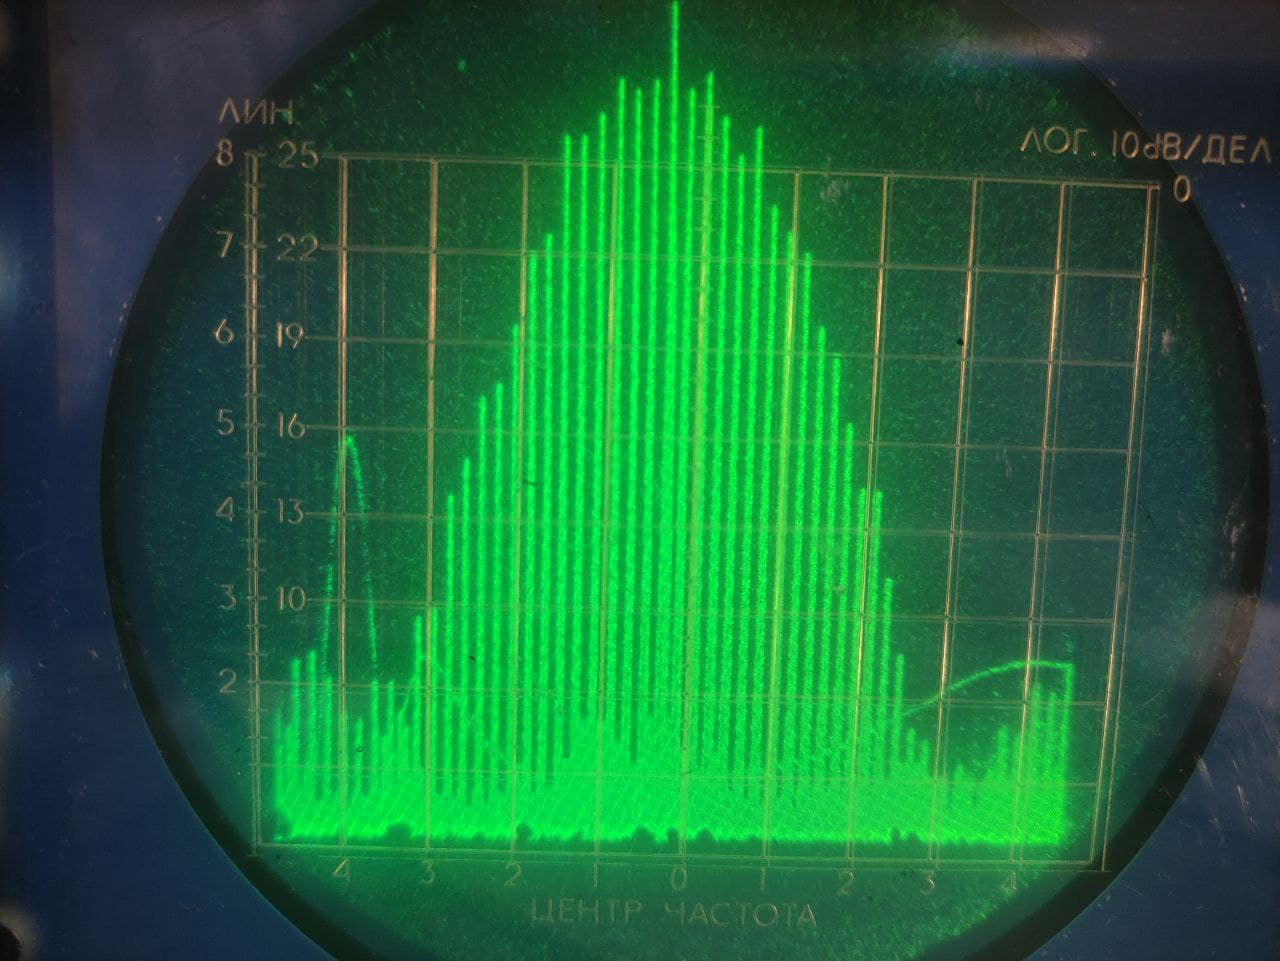
\includegraphics[scale=0.2]{images/50_1000_25-b.jpg}
\caption{$f_{\text{повт}} = 10^3$ Гц, $\tau = 50$ мкс, $\nu_0 = 25$ кГц}
\label{fig:Image1}
\end{figure}

\begin{figure}[h!]
\centering
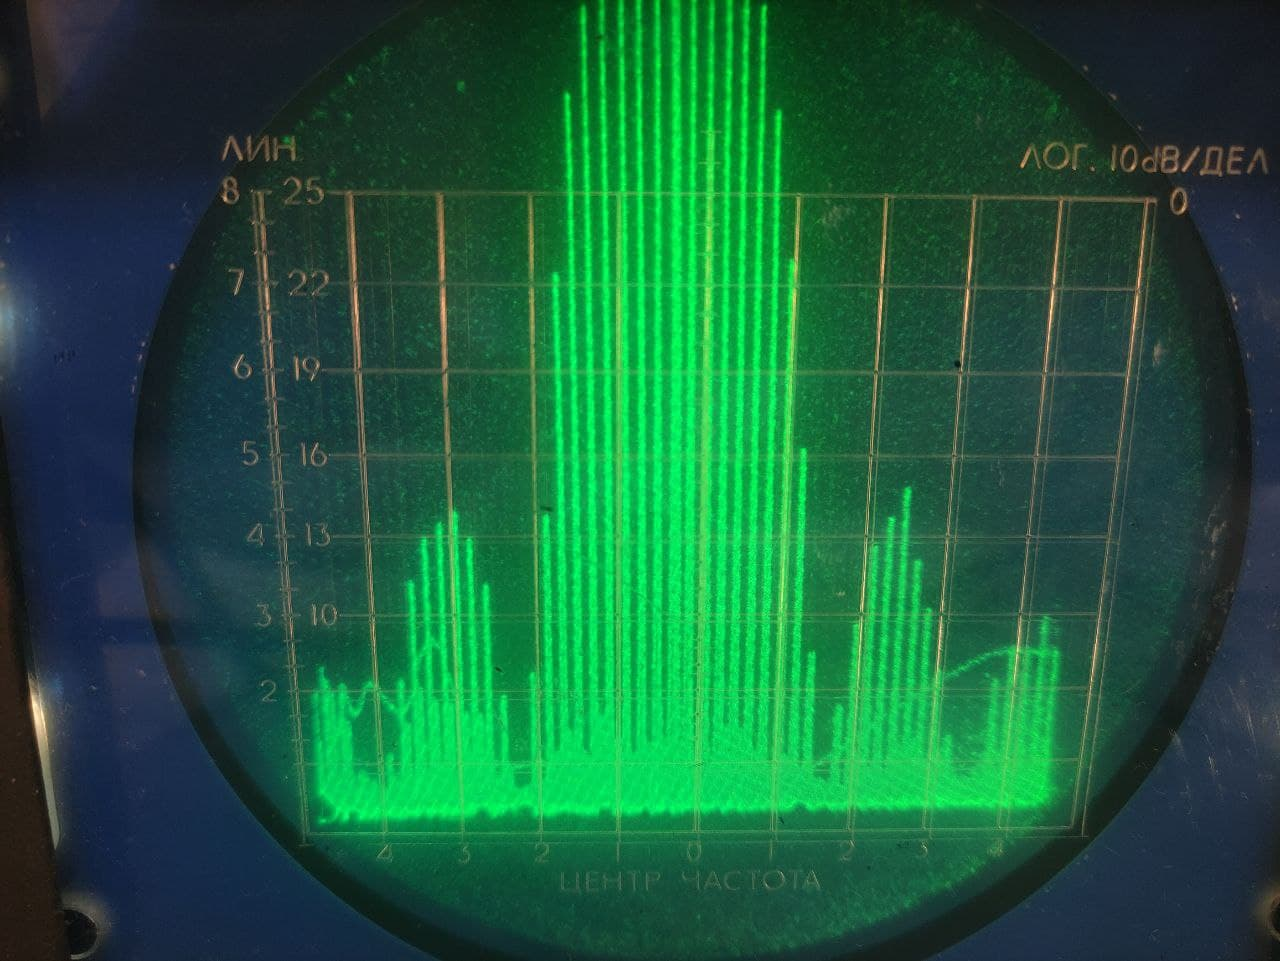
\includegraphics[scale=0.2]{images/100_1000_25-b.jpg}
\caption{$f_{\text{повт}} = 10^3$ Гц, $\tau = 100$ мкс, $\nu_0 = 25$ кГц}
\label{fig:Image1}
\end{figure}

\begin{figure}[h!]
\centering
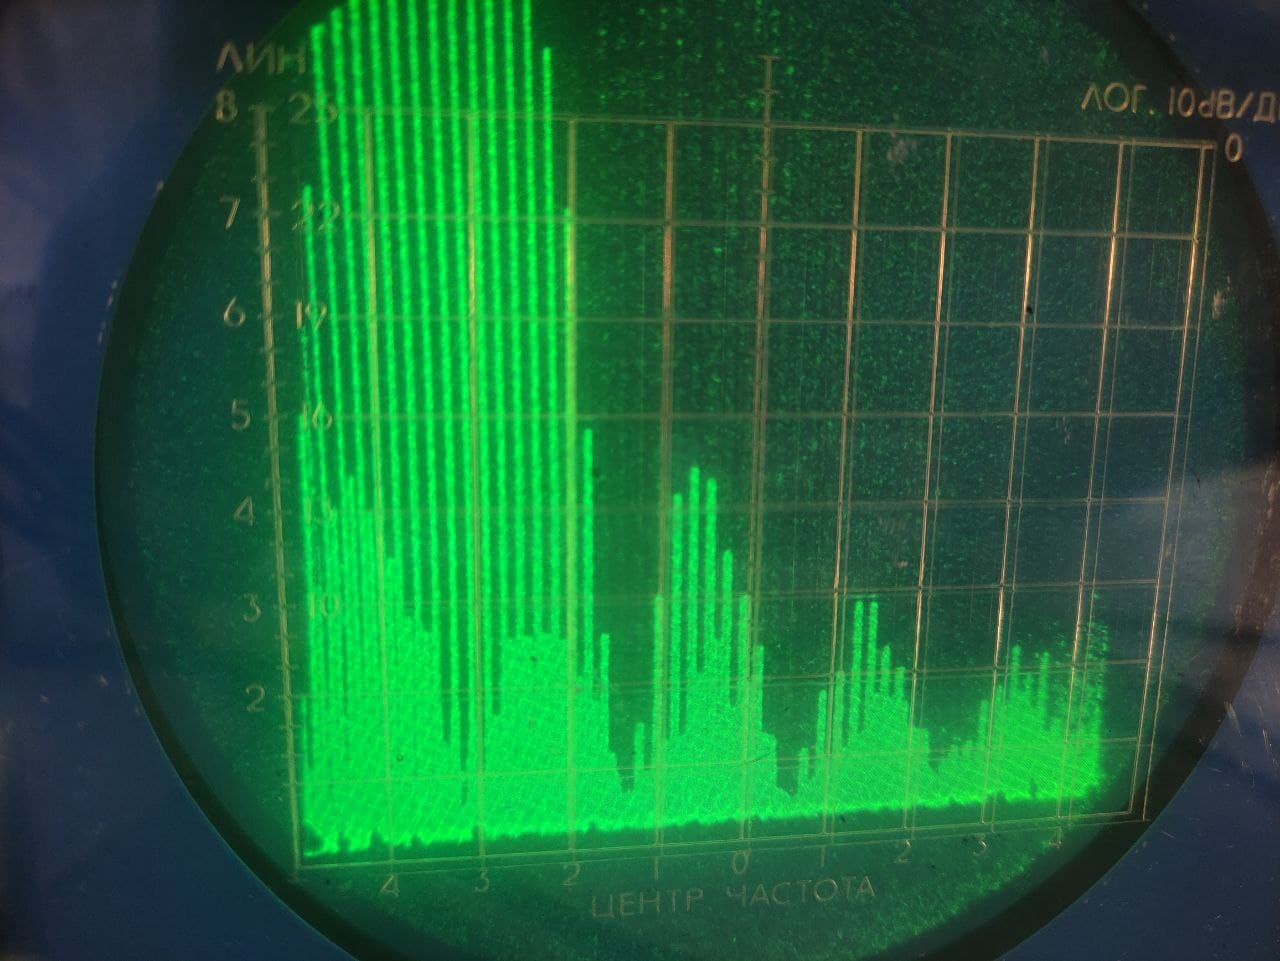
\includegraphics[scale=0.2]{images/100_1000_10-b.jpg}
\caption{$f_{\text{повт}} = 10^3$ Гц, $\tau = 100$ мкс, $\nu_0 = 10$ кГц}
\label{fig:Image1}
\end{figure}

\begin{figure}[h!]
\centering
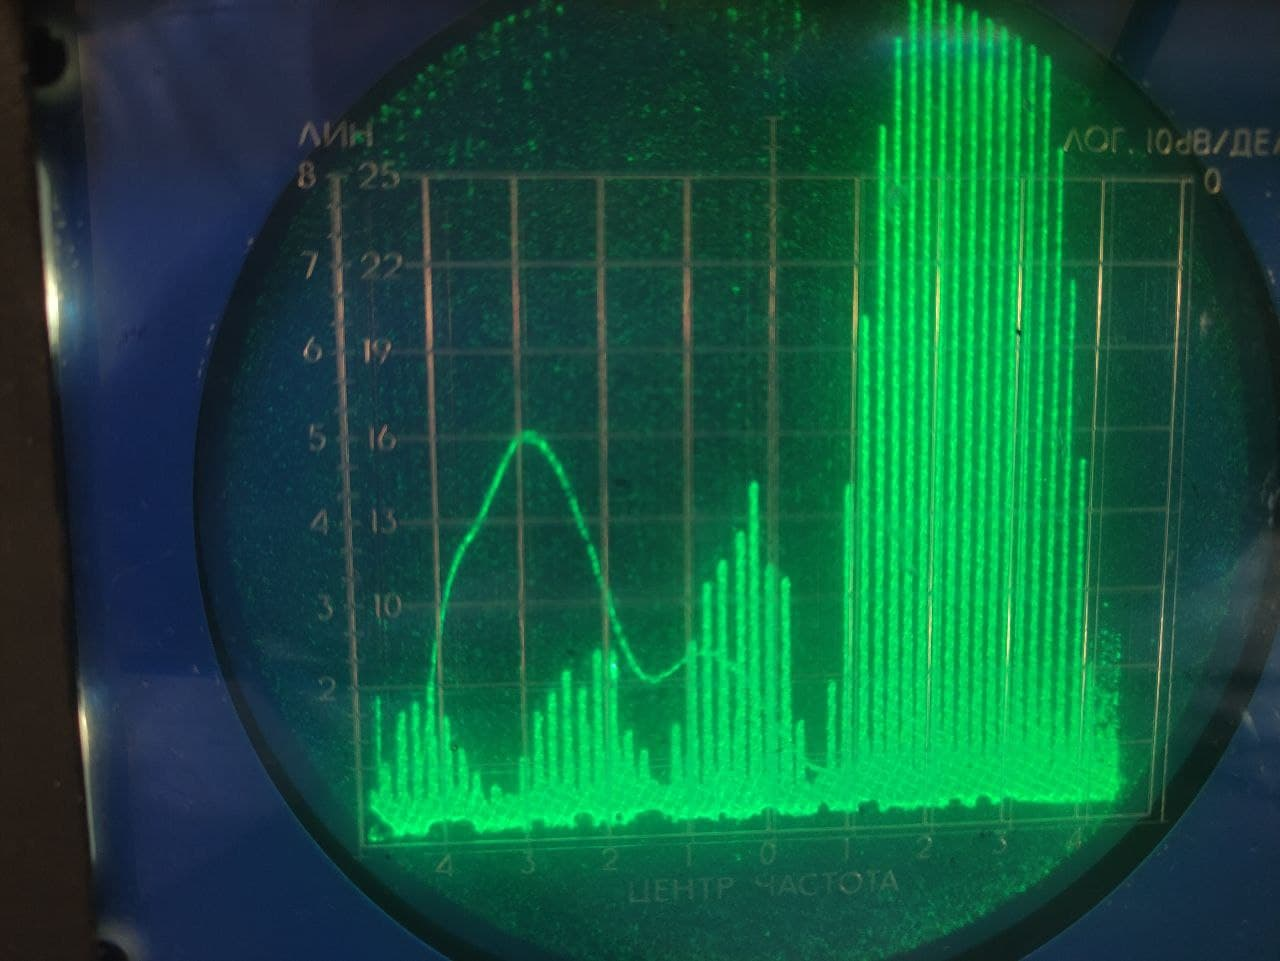
\includegraphics[scale=0.2]{images/100_1000_40-b.jpg}
\caption{$f_{\text{повт}} = 10^3$ Гц, $\tau = 100$ мкс, $\nu_0 = 40$ кГц}
\label{fig:Image1}
\end{figure}

\newpage

\item  При фиксированной длительности импульсов $\tau = 50$ мкс исследуем зависимость расстояния $\delta \nu$ между соседними спектральными компонентами от периода $T$ (частоты повторения импульсов $f_{\text{повт}}$). Запишем данные в таблицу:

\begin{figure}[h!]
\centering
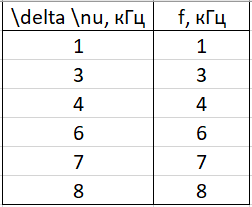
\includegraphics[scale=1.2]{images/table2.png}
\caption{Зависимость $\delta \nu (T)$}
\label{fig:Image1}
\end{figure}

\newpage

\item Посмотрим на спектры цугов с параметрами $\tau = 100$ мкс, $m_x = 5$ кГц/дел:

а)$f_{\text{повт}} = 1$ кГц

б)$f_{\text{повт}} = 2$ кГц

\begin{figure}[h!]
\centering
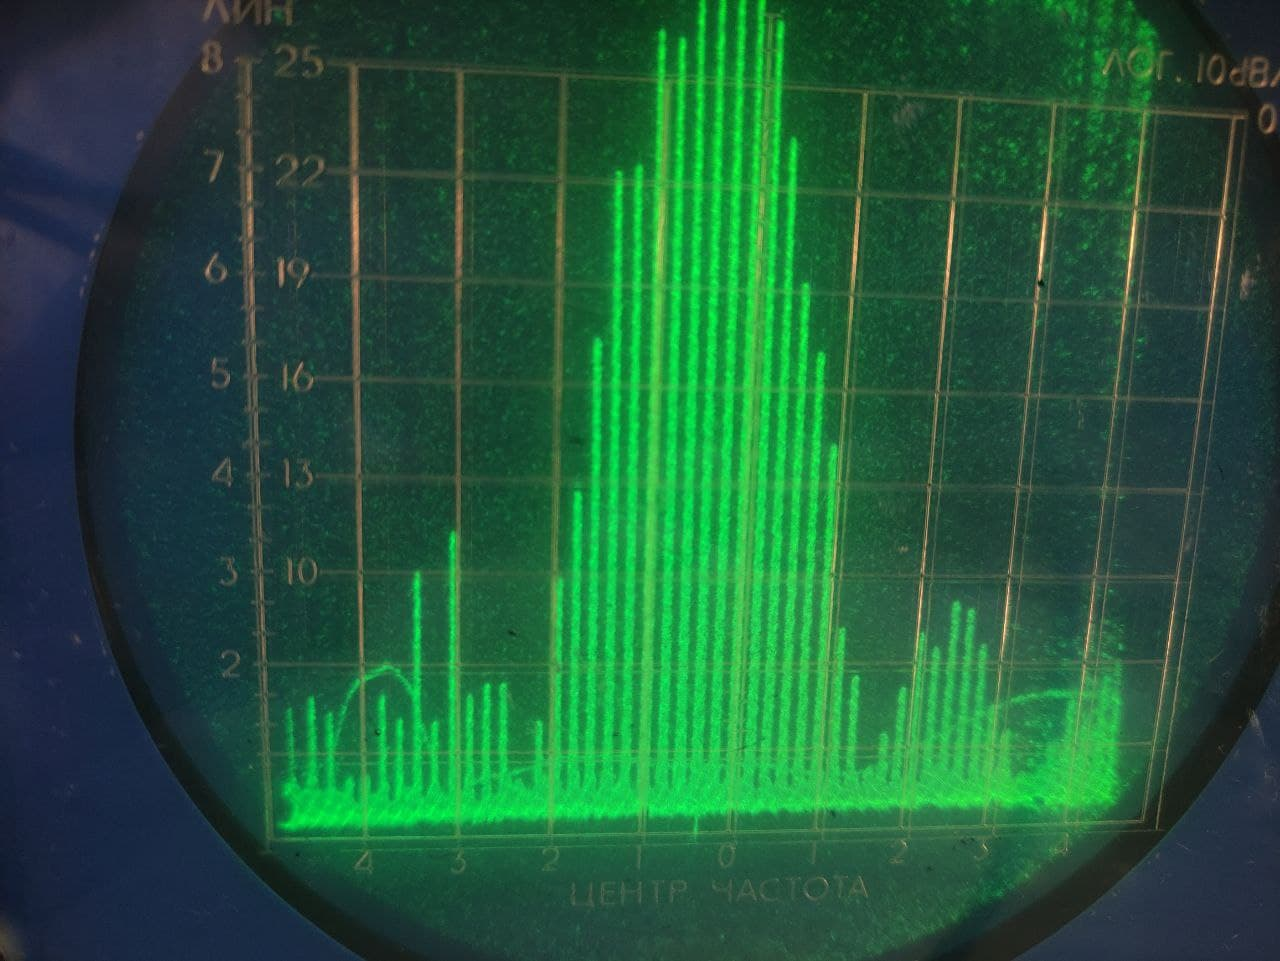
\includegraphics[scale=0.2]{images/100_1000_25-b2.jpg}
\caption{$f_{\text{повт}} = 10^3$ Гц, $\tau = 100$ мкс, $\nu_0 = 25$ кГц}
\label{fig:Image1}
\end{figure}

\begin{figure}[h!]
\centering
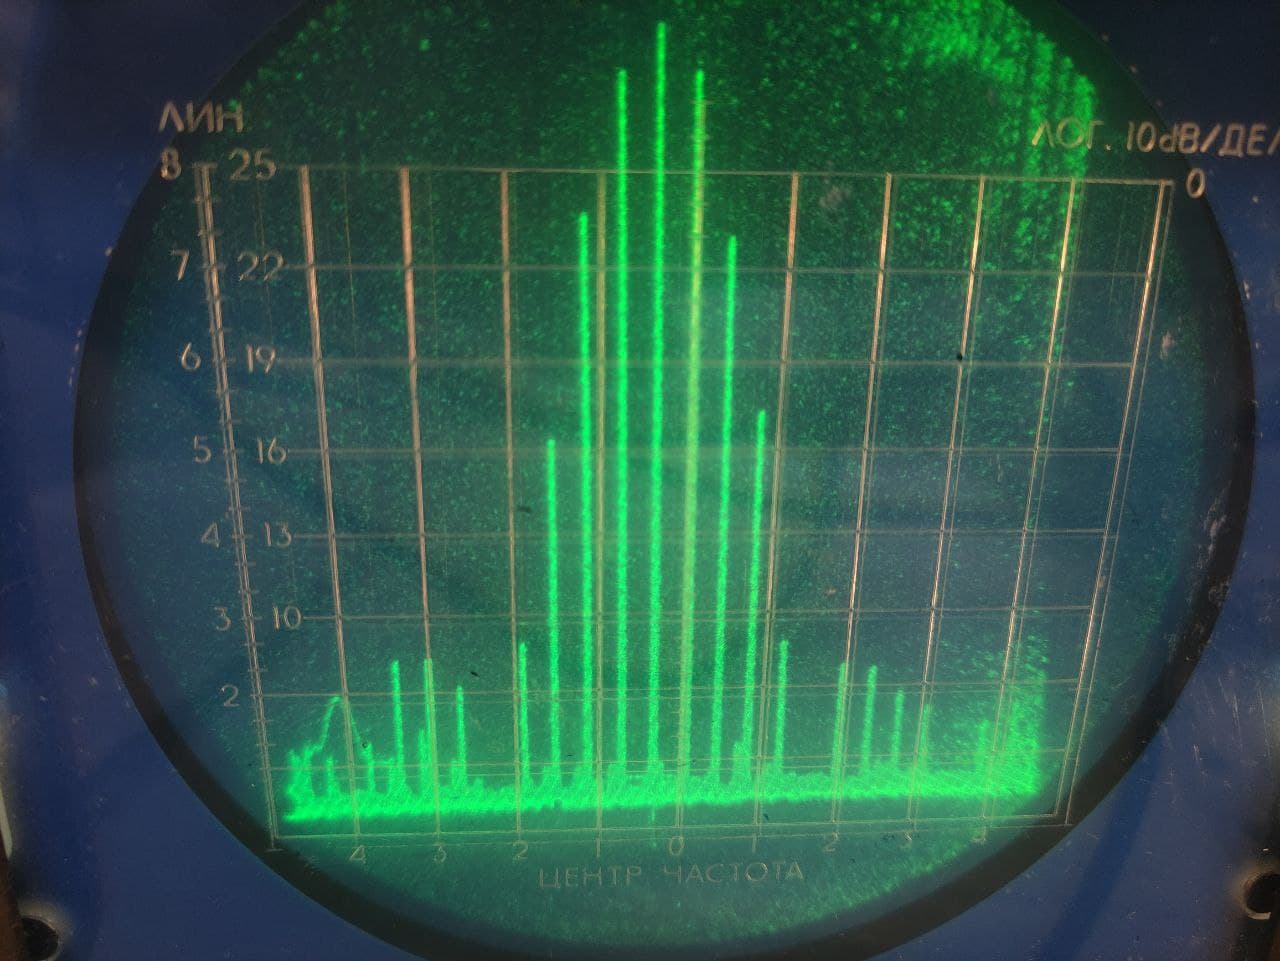
\includegraphics[scale=0.2]{images/100_2000_25-b.jpg}
\caption{$f_{\text{повт}} = 2\cdot 10^3$ Гц, $\tau = 100$ мкс, $\nu_0 = 25$ кГц}
\label{fig:Image1}
\end{figure}

\newpage

\item Построим график $\delta \nu (f_{\text{повт}})$:

\begin{figure}[h!]
\centering
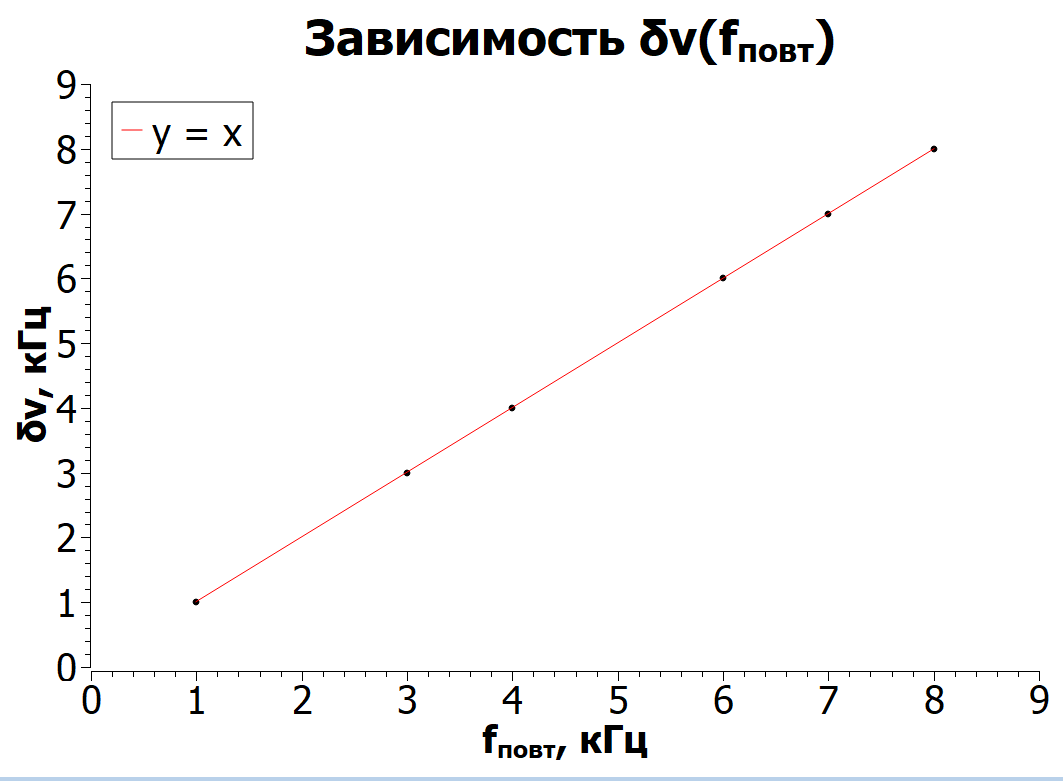
\includegraphics[scale=0.8]{images/graph2.png}
\label{fig:Image1}
\end{figure}

\end{enumerate}

\newpage

\subsection*{В}

\begin{enumerate}

\item Соберем схему изображенную на рисунке.

\begin{figure}[h!]
\centering
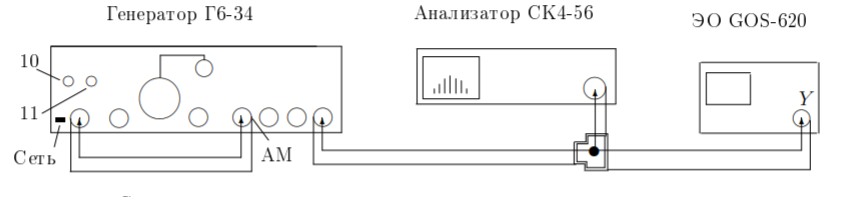
\includegraphics[scale=0.6]{images/scheme2.png}
\label{fig:Image1}
\end{figure}

\item Изменяя глубину модуляции исследуем зависимость отношения амплитуды боковой линии спектра к амплитуде основной линии ($a_{\text{бок}}/a_{\text{осн}}$) от глубины модуляции $m$, вычисляемой по формуле:

\[m = \frac{A_{max} - A_{min}}{A_{max} + A_{min}}\]

Запишем данные в таблицу:

\begin{figure}[h!]
\centering
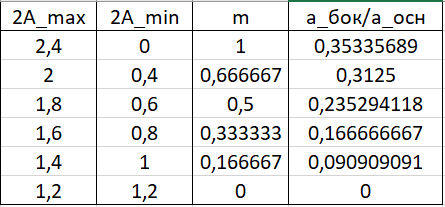
\includegraphics[scale=1.2]{images/table3.png}
\caption{Зависимость $a_{\text{бок}/a_{\text{осн}}} = f(m)$}
\label{fig:Image1}
\end{figure}

\item По полученным данным построим график $a_{\text{бок}/a_{\text{осн}}} = f(m)$: $\pm$

\begin{figure}[h!]
\centering
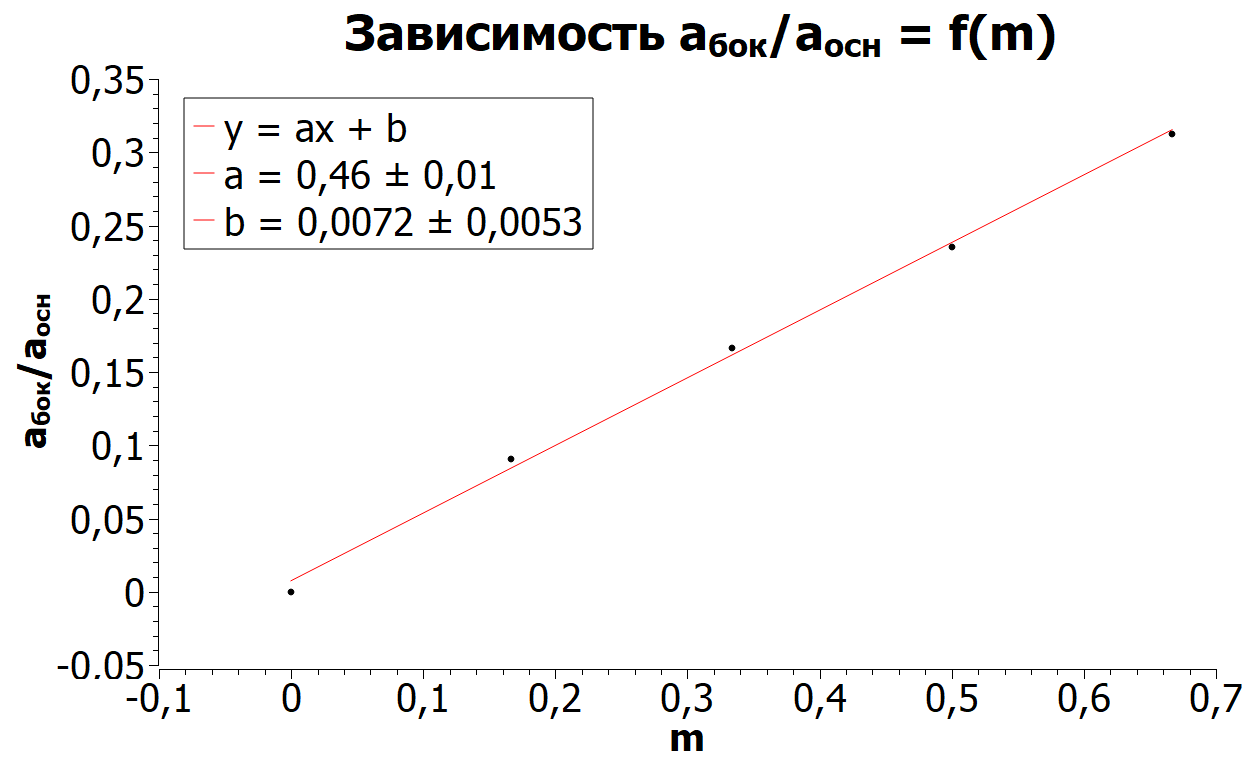
\includegraphics[scale=0.8]{images/graph3.png}
\label{fig:Image1}
\end{figure}

Получаем значение углового коэффициента наклона:

\[a = 0,46 \pm 0,01,\]

что примерно совпадает с теоретическим значением для данной величины.

\end{enumerate}

\end{document}